\documentclass[tikz,border=7pt]{standalone}
\usetikzlibrary{calc}
\begin{document}
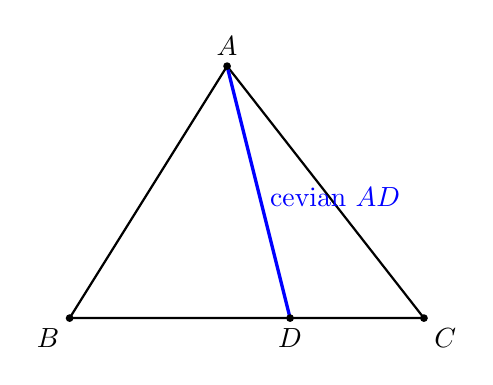
\begin{tikzpicture}[line width=.8pt]
\coordinate (A) at (0,3.2); \coordinate (B) at (-2,0); \coordinate (C) at (2.5,0); \coordinate (D) at (.8,0);
\draw (A)--(B)--(C)--cycle; \draw[blue,very thick] (A)--(D);
\foreach \p/\pos in {A/above,B/below left,C/below right,D/below} \fill (\p) circle (1.4pt) node[\pos] {$\p$};
\node[blue,right] at ($(A)!.52!(D)$) {cevian $AD$};
\end{tikzpicture}
\end{document}
